\documentclass[a4paper, titlepage]{article}
\usepackage[T1]{fontenc}
\usepackage[utf8]{inputenc}
\usepackage[italian]{babel}
\usepackage{geometry}
\usepackage{graphicx}
\geometry{a4paper,top=3cm,bottom=3cm,left=3cm,right=3cm,%
heightrounded,bindingoffset=5mm}
% commenti su più righe
\usepackage{verbatim}
% librerie per tabelle
\usepackage{lscape}
\usepackage{longtable}
\usepackage{booktabs}
\usepackage[normalem]{ulem}
\useunder{\uline}{\ul}{}
\begin{document}

% Frontespizio
\begin{titlepage}
\centering
\vspace{5cm}
{\LARGE\bfseries Universit\`a degli Studi di Milano-Bicocca\par}
\vspace{1ex}
\hrule
\vspace{1ex}
Dipartimento di Informatica, Sistemistica e Comunicazione\\
Corso di Laurea Triennale in Informatica\\
\vspace{6cm}
Documentazione di progetto\\
\vspace{1cm}
{\Huge \bfseries \scshape Brew Day!\par}
\vspace{6cm}
\begin{tabular*}{\textwidth}{@{}l@{\extracolsep{\fill}}l@{}}
Alessia Calzari,   a.calzari@campus.unimib.it\\
Matricola: 844884\\
\\
Dario Gianotti,   d.gianotti2@campus.unimib.it\\
Matricola: 847052\\
\\
Andrea Provasi,   a.provasi2@campus.unimib.it\\
Matricola: 847015\\
\\
Riccardo Riva,   r.riva36@campus.unimib.it\\
Matricola: 844936
\end{tabular*}
\vspace{\fill}
\hrule
\vspace{1ex}
\centering
\textbf{Anno Accademico 2020-2021}
\end{titlepage}

% Sommario
\tableofcontents

\newpage
L'obiettivo di questo progetto è quello di sviluppare un'applicazione per i produttori di birra artigianale.\\
L'applicazione permette la registrazione degli utenti per salvare le proprie ricette, segnare l'elenco dei prodotti disponibili e la propria attrezzatura.\\
In questo modo l'utente potrà effettuare il login con le proprie credenziali per effettuare diverse operazioni:
\begin{itemize}
    \item modificare il proprio account o eliminarlo
    \item aggiungere una nuova ricetta (con prodotti, attrezzatura necessaria, preparazione e note) o eliminarne una dalla lista delle ricette
    \item modificare una ricetta (ad esempio aggiornare le note)
    \item aggiungere, rimuovere o modificare un attrezzo dalla lista delle attrezzature
    \item aggiungere o rimuovere un prodotto alla lista dei prodotti
    \item modificare un prodotto (ad esempio la quantità dopo aver fatto la spesa)
    \item consultare la lista della spesa che contiene tutti i prodotti utilizzati e le loro quantità, avrà anche la possibilità di esportare questa lista per modificarla a piacimento
    \item scegliere la ricetta della birra da preparare ed indicarne la quantità, una volta selezionato questo gli ingredienti utilizzati saranno aggiunti alla lista della spesa
    \item usare la funzionalità "Che birra faccio?" che mostrerà la ricetta che massimizza l'utilizzo degli ingredienti disponibili
\end{itemize}

\newpage
\section{Analisi}
\subsection{Casi d'uso}
Abbiamo identificato 8 casi d'uso che di seguito abbiamo illustrato nella forma dettagliata.
\vphantom{}
\subsection{Diagramma dei casi d'uso}
\vphantom{}
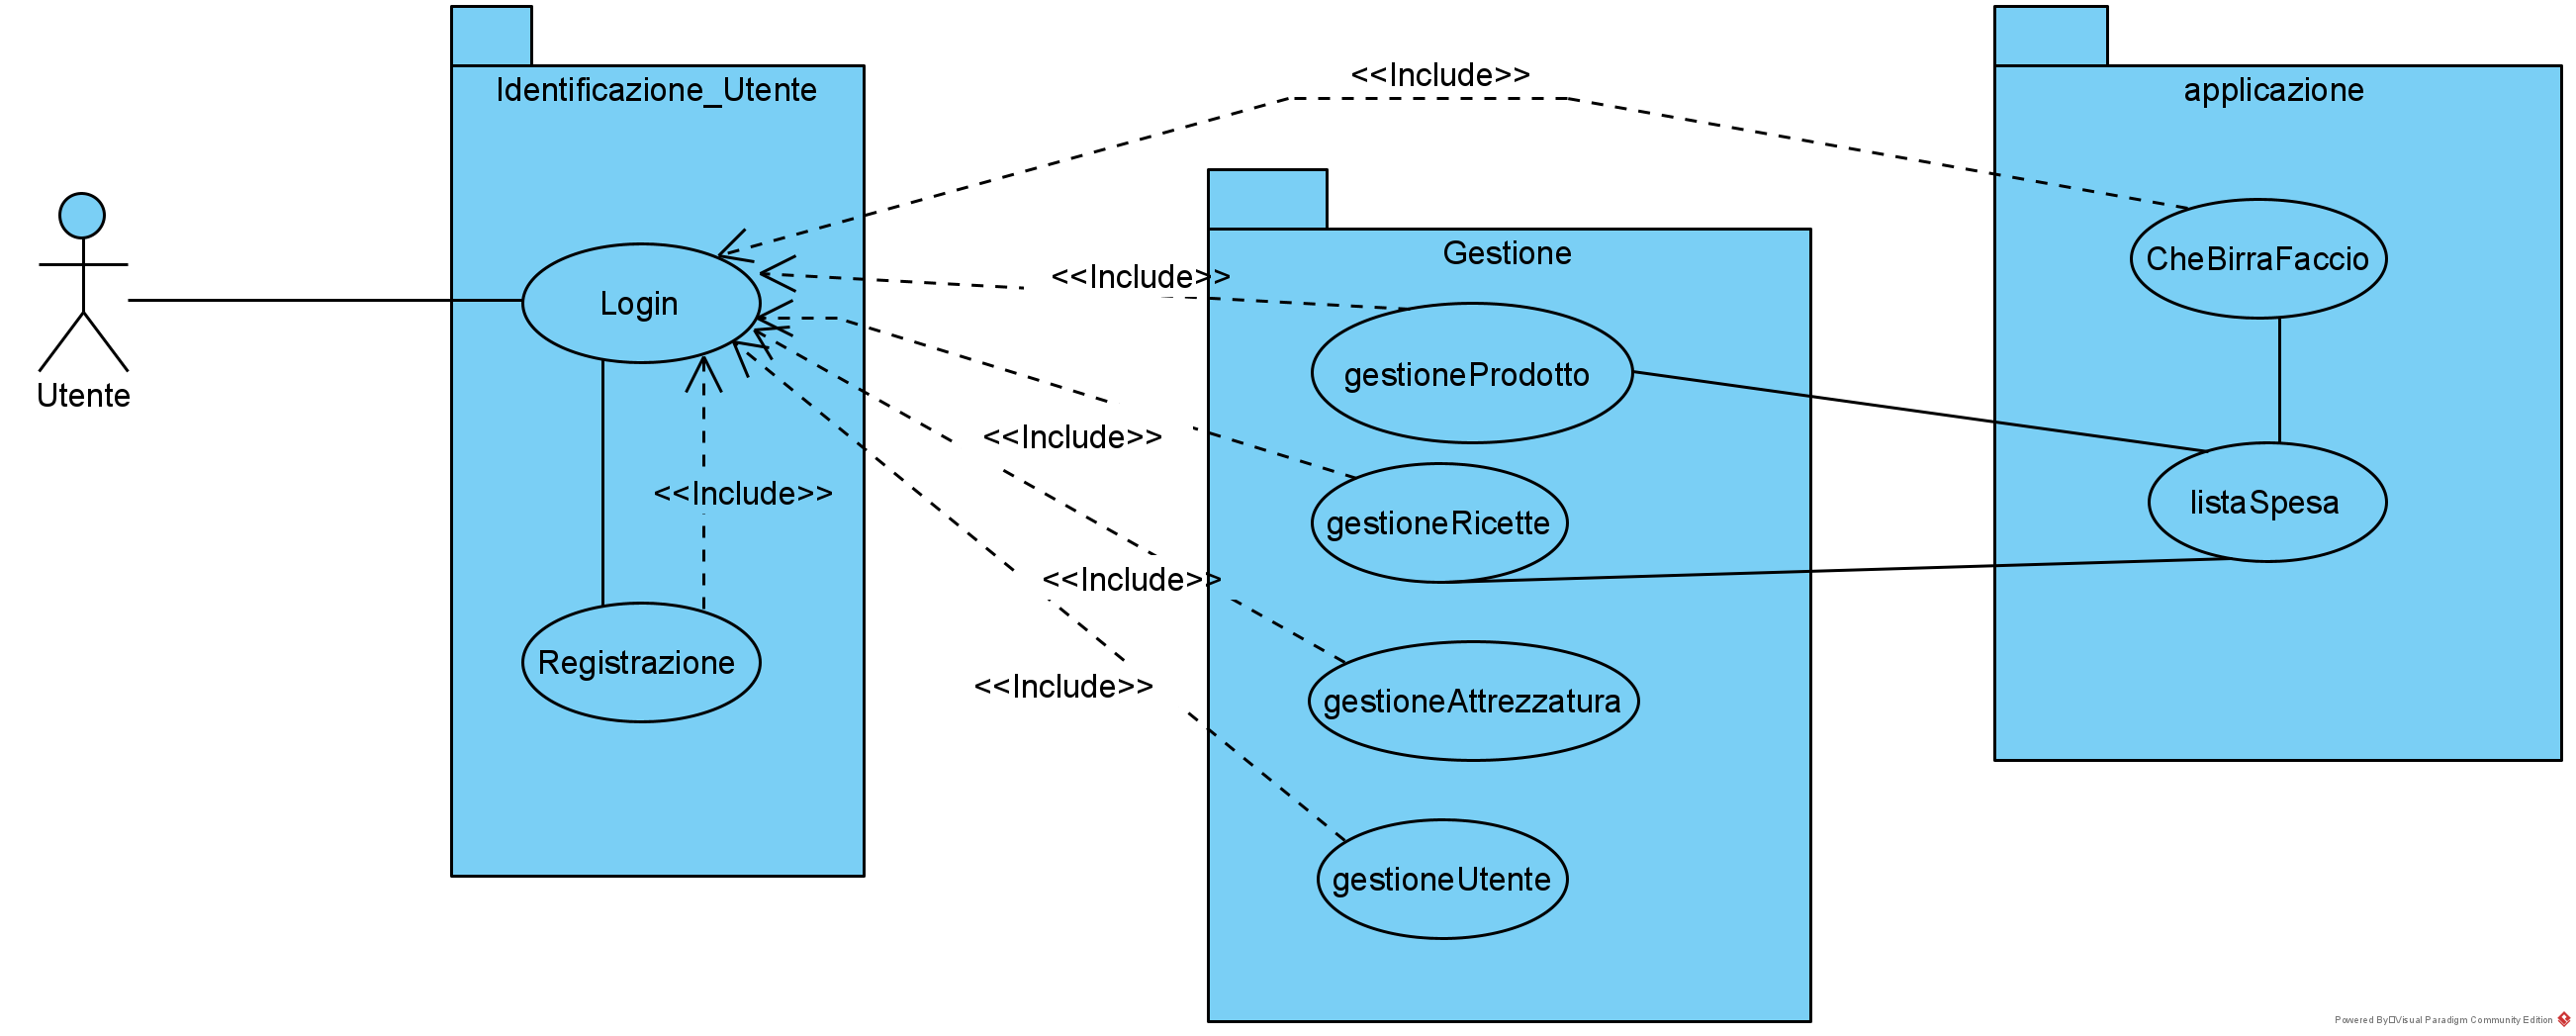
\includegraphics[scale=0.65]{Immagini/Use Case Diagram_Brew Day!.png}
\vphantom{}
\subsubsection{Login}
\begin{longtable}{p{6cm}p{7cm}}\toprule
    NOME & Login\\\midrule
    PORTATA & Brew Day!\\\midrule
    LIVELLO & Gestione di ricette di birre artigianali\\\midrule
    ATTORE PRIMARIO & Utente\\\midrule
    PARTI INTERESSATE E INTERESSI & L’attore Utente vuole accedere al sito “Brew Day!” inserendo le proprie credenziali\\\midrule
    PRE-CONDIZIONI & L’attore Utente deve aver effettuato la registrazione\\\midrule
    GARANZIA DI SUCCESSO & L’attore Utente riesce ad accedere al sito di “Brew Day!”\\\midrule
    SCENARIO PRINCIPALE DI
    & 1) il sistema visualizza la schermata login\\
    SUCCESSO & 2) l’utente inserisce le credenziali\\
    & 3) il sistema verifica la correttezza
    dei dati sul database\\\midrule
    ESTENSIONI &
    3.1) in caso di dati corretti viene effettuato il login\\
    & 3.2) in caso di dati errati il sistema
    visualizza un messaggio di errore\\\midrule
    REQUISITI SPECIALI & Nessuno \\\midrule
    ELENCO VARIABILI TECNOLOGICHE & Database\\\midrule
    FREQUENZA DI RIPETIZIONE & Più volte al giorno\\\midrule
    VARIE & Nessuna\\\bottomrule
\end{longtable}
\vphantom{}
\newpage
\subsubsection{Registrazione}
\begin{longtable}{p{6cm}p{7cm}}\toprule
    NOME & Registrazione\\\midrule
    PORTATA & Brew Day!\\\midrule
    LIVELLO & Gestione di ricette di birra artigianali\\\midrule
    ATTORE PRIMARIO & Utente\\\midrule
    PARTI INTERESSATE E INTERESSI & L’attore Utente vuole registrarsi al sito di “Brew Day!" inserendo e-mail e password\\\midrule
    PRE-CONDIZIONI & Nessuna\\\midrule
    GARANZIA DI SUCCESSO & L’attore Utente riesce ad effettuare la registrazione\\\midrule
    SCENARIO PRINCIPALE DI
    & 1) l’utente preme su "Crea Account"\\
    SUCCESSO & 2) il sistema visualizza la schermata di registrazione (e-mail e password)\\
    & 3) l’utente inserisce i propri dati\\
    & 4) il sistema   verifica la correttezza dei dati inseriti\\\midrule
    ESTENSIONI
    & 4.1) in caso di dati corretti essi vengono inseriti
    nel database ed il sistema visualizza un messaggio di successo\\
    & 4.2) in caso di dati errati viene visualizzato un messaggio di errore ed il cliente può reinserire i dati\\\midrule
    REQUISITI SPECIALI & Nessuno\\\midrule
    ELENCO VARIABILI TECNOLOGICHE & Database\\\midrule
    FREQUENZA DI RIPETIZIONE & Una volta per utente\\\midrule
    VARIE & Nessuna\\\bottomrule                                
\end{longtable}
\vphantom{}
\newpage
\subsubsection{gestioneUtente}
\begin{longtable}{p{6cm}p{7cm}}\toprule
    NOME & gestioneUtente\\\midrule
    PORTATA & Brew Day!\\\midrule
    LIVELLO & Gestione di ricette di birra artigianali\\\midrule
    ATTORE PRIMARIO & Utente\\\midrule
    PARTI INTERESSATE E INTERESSI & L’attore Utente vuole visualizzare il proprio profilo, modificare informazioni o eliminarlo\\\midrule
    PRE-CONDIZIONI & Login\\\midrule
    GARANZIA DI SUCCESSO & L’attore Utente riesce a visualizzare il proprio profilo, modificare informazioni o eliminarlo\\\midrule
    SCENARIO PRINCIPALE DI
    & 1) l’utente seleziona la voce "Profilo"\\
    SUCCESSO & 2) il sistema restituisce la schermata con i dati del profilo\\
    & 3.1) l’utente seleziona “modifica profilo”\\
    & 3.2) l’utente seleziona “elimina profilo”\\
    & 4.1) il sistema restituisce la schermata di modifica del profilo\\
    & 4.2) il sistema visualizza una schermata di conferma eliminazione\\
    & 5.1) l’utente modifica i dati desiderati e preme “salva”\\
    & 5.2) l’utente preme su “elimina”\\
    & 6.1) il sistema salva il nuovi dati nel database e restituisce un messaggio di conferma\\
    & 6.2) il sistema elimina i dati relativi dal database e restituisce un messaggio di conferma\\\midrule
    ESTENSIONI
    & 6.1.1) se il profilo non viene salvato correttamente, il sistema restituisce un messaggio di errore\\
    & 6.2.1) se il profilo non viene eliminato correttamente, il sistema restituisce un messaggio di errore\\\midrule
    REQUISITI SPECIALI & Nessuno\\\midrule
    ELENCO VARIABILI TECNOLOGICHE & Database\\\midrule
    FREQUENZA DI RIPETIZIONE & Più volte al giorno\\\midrule
    VARIE & Nessuna\\\bottomrule
\end{longtable}
\newpage
\subsubsection{gestioneProdotto}
\begin{longtable}{p{6cm}p{7cm}}\toprule
    NOME & gestioneProdotto\\\midrule
    PORTATA & Brew Day!\\\midrule
    LIVELLO & Gestione di ricette di birra artigianali\\\midrule
    ATTORE PRIMARIO & Utente\\\midrule
    PARTI INTERESSATE E INTERESSI & L’attore Utente vuole visualizzare la lista dei prodotti, modificare, aggiungere o rimuovere i prodotti che ha in casa\\\midrule
    PRE-CONDIZIONI & Login\\\midrule
    GARANZIA DI SUCCESSO &  L’attore Utente riesce a visualizzare la lista dei prodotti, modificare, aggiungere o rimuovere i prodotti che ha in casa\\\midrule
    SCENARIO PRINCIPALE DI
    & 1) l’utente seleziona la voce prodotti\\
    SUCCESSO & 2) il sistema restituisce la lista dei prodotti\\
    & 3.1) l’utente seleziona “aggiungi prodotto”\\
    & 3.2) l’utente seleziona “modifica prodotto”\\
    & 3.3) l’utente seleziona “elimina prodotto”\\
    & 4.1) il sistema restituisce la schermata per aggiungere il prodotto\\
    & 4.2) il sistema restituisce la schermata di ricerca del prodotto da modificare\\
    & 4.3) il sistema restituisce la schermata di ricerca del prodotto da eliminare\\
    & 5.1) l’utente inserisce i dati del prodotto e preme “salva”\\
    & 5.2) l’utente inserisce i dati del prodotto e preme “cerca”\\
    & 5.3) l’utente inserisce i dati del prodotto e preme “cerca”\\
    & 6.1) il sistema salva il nuovo prodotto nel database e restituisce un messaggio di conferma\\
    & 6.2) il sistema restituisce i prodotti che coincidono con la ricerca\\
    & 6.3) il sistema restituisce i prodotti che coincidono con la ricerca\\
    & 7.2) l’utente seleziona il prodotto desiderato e preme su “modifica”\\
    & 7.3) l’utente seleziona il prodotto desiderato e preme su “elimina”\\
    & 8.2) il sistema visualizza i dati modificabili relativi al prodotto selezionato\\
    & 8.3) il sistema visualizza una schermata di conferma eliminazione\\
    & 9.2) l’utente modifica i dati che desidera e preme su “salva”\\
    & 9.3) l’utente preme su “elimina”\\
    & 10.2) il sistema salva il nuovi dati nel database e restituisce un messaggio di conferma\\
    & 10.3) il sistema elimina i dati relativi al prodotto dal database e restituisce un messaggio di conferma\\\\\\\\\midrule
    ESTENSIONI
    & 6.1.1) se il prodotto non viene salvato correttamente, il sistema restituisce un messaggio di errore\\
    & 10.2.1) se il prodotto non viene salvato correttamente, il sistema restituisce un messaggio di errore\\
    & 10.3.1) se il prodotto non viene eliminato correttamente, il sistema restituisce un messaggio di errore \\\midrule
    REQUISITI SPECIALI & Nessuno\\\midrule
    ELENCO VARIABILI TECNOLOGICHE & Database\\\midrule
    FREQUENZA DI RIPETIZIONE & Più volte al giorno\\\midrule
    VARIE & Nessuna\\\bottomrule
\end{longtable}
\vphantom{}
\subsubsection{gestioneAttrezzatura}
\begin{longtable}{p{6cm}p{7cm}}\toprule
    NOME & gestioneAttrezzatura\\\midrule
    PORTATA & Brew Day!\\\midrule
    LIVELLO & Gestione di ricette di birra artigianali\\\midrule
    ATTORE PRIMARIO & Utente\\\midrule
    PARTI INTERESSATE E INTERESSI &
    L’attore Utente vuole visualizzare la lista dell’attrezzatura, aggiungere o rimuovere attrezzatura che ha in casa \\\midrule
    PRE-CONDIZIONI & Login\\\midrule
    GARANZIA DI SUCCESSO & L’attore Utente riesce a visualizzare la lista dell’attrezzatura, aggiungere o rimuovere
    attrezzatura che ha in casa\\\midrule
    SCENARIO PRINCIPALE DI
    & 1) l’utente seleziona la voce attrezzatura\\
    SUCCESSO & 2) il sistema restituisce la lista dell’attrezzatura\\
    & 3.1) l’utente seleziona “aggiungi attrezzatura”\\
    & 3.2) l’utente seleziona “elimina attrezzatura”\\
    & 4.1) il sistema restituisce la schermata per aggiungere un attrezzo\\
    & 4.2) il sistema restituisce la schermata di ricerca dell’attrezzo da eliminare\\
    & 5.1) l’utente inserisce i dati dell’attrezzo e preme “salva”\\
    & 5.2) l’utente inserisce i dati dell’attrezzo e preme “cerca”\\
    & 6.1) il sistema salva il nuovo attrezzo ne database e restituisce un messaggio di conferma\\
    & 6.2) il sistema restituisce gli attrezzi che coincidono con la ricerca\\
    & 7.2) l’utente seleziona l’attrezzo desiderato e preme su “elimina”\\
    & 8.2) il sistema visualizza una schermata di conferma eliminazione\\
    & 9.2) l’utente preme su “elimina”\\
    & 10.2) il sistema elimina i dati relativi al prodotto dal database e restituisce un messaggio di conferma\\\midrule
    ESTENSIONI
    & 6.1.1) se l’attrezzo non viene salvato correttamente, il sistema restituisce un messaggio di errore\\
    & 10.2.1) se l’attrezzo non viene eliminato correttamente, il sistema restituisce un messaggio di errore\\\midrule
    REQUISITI SPECIALI & Nessuno\\\midrule
    ELENCO VARIABILI TECNOLOGICHE & Database\\\midrule
    FREQUENZA DI RIPETIZIONE & Più volte al giorno\\\midrule
    VARIE & Nessuna\\\bottomrule
\end{longtable}
\vphantom{}
\subsubsection{gestioneRicette}
\begin{longtable}{p{6cm}p{7cm}}\toprule
    NOME & gestioneRicette\\\midrule
    PORTATA & Brew Day!\\\midrule
    LIVELLO & Gestione di ricette di birra artigianali\\\midrule
    ATTORE PRIMARIO & Utente\\\midrule
    PARTI INTERESSATE E INTERESSI &
    L’attore Utente vuole visualizzare la lista delle ricette, modificare, aggiungere o rimuovere i prodotti che ha in casa \\\midrule
    PRE-CONDIZIONI & Login\\\midrule
    GARANZIA DI SUCCESSO & L’attore Utente riesce a visualizzare la lista delle ricette, modificare, aggiungere o rimuovere i prodotti che ha in casa \\\midrule
    SCENARIO PRINCIPALE DI
    & 1) l’utente seleziona la voce ricette\\
    SUCCESSO & 2) il sistema restituisce la lista delle ricette\\
    & 3.1) l’utente seleziona “aggiungi ricetta”\\
    & 3.2) l’utente seleziona “modifica ricetta”\\
    & 3.3) l’utente seleziona “elimina ricetta”\\
    & 3.4) l'utente seleziona "prepara ricetta"\\
    & 4.1) il sistema restituisce la schermata per aggiungere la ricetta\\
    & 4.2) il sistema restituisce la schermata di ricerca della ricetta da modificare\\
    & 4.3) il sistema restituisce la schermata di ricerca della ricetta da eliminare\\
    & 4.4) il sistema visualizza la preparazione della ricetta (ingredienti, procedimento)\\
    & 5.1) l’utente inserisce i dati della ricetta e preme “salva”\\
    & 5.2) l’utente inserisce i dati della ricetta e preme “cerca”\\
    & 5.3) l’utente inserisce i dati della ricetta e preme “cerca”\\
    & 5.4) l'utente preme su "prepara"\\
    & 6.1) il sistema salva la nuova ricetta nel database e restituisce un messaggio di conferma\\
    & 6.2) il sistema restituisce le ricette che coincidono con la ricerca\\
    & 6.3) il sistema restituisce le ricette che coincidono con la ricerca\\
    & 6.4) il sistema chiede quanti litri preparare\\
    & 7.2) l’utente seleziona la ricetta desiderata e preme su “modifica”\\
    & 7.3) l’utente seleziona la ricetta desiderata e preme su “elimina”\\
    & 7.4) l'utente inserisce la quantità di birra da preparare e preme su "ok"\\
    & 8.2) il sistema visualizza i dati modificabili relativi alla ricetta selezionata\\
    & 8.3) il sistema visualizza una schermata di conferma eliminazione\\
    & 8.4) il sistema sposta dalla lista dei prodotti alla lista della spesa la quantità di prodotti utilizzata per la preparazione della ricetta\\
    & 9.2) l’utente modifica i dati che desidera e preme su “salva”\\
    & 9.3) l’utente preme su “elimina”\\
    & 10.2) il sistema salva il nuovi dati nel database e restituisce un messaggio di conferma\\
    & 10.3) il sistema elimina i dati relativi alla ricetta dal database e restituisce un messaggio di conferma\\\midrule
    ESTENSIONI
    & 6.1.1) se la ricetta non viene salvata correttamente, il sistema restituisce un messaggio di errore\\
    & 10.2.1) se la ricetta non viene salvata correttamente, il sistema restituisce un messaggio di errore\\
    & 10.3.1) se la ricetta non viene eliminata correttamente, il sistema restituisce un messaggio di errore\\
    & 8.4.1) se non ho le quantità sufficienti di prodotti necessari alla preparazione, il sistema restituisce un messaggio di errore\\\midrule
    REQUISITI SPECIALI & Nessuno\\\midrule
    ELENCO VARIABILI TECNOLOGICHE & Database\\\midrule
    FREQUENZA DI RIPETIZIONE & Più volte al giorno\\\midrule
    VARIE & Nessuna\\\bottomrule
\end{longtable}
\vphantom{}
\subsubsection{listaSpesa}
\begin{longtable}{p{6cm}p{7cm}}\toprule
    NOME & listaSpesa\\\midrule
    PORTATA & Brew Day!\\\midrule
    LIVELLO & Gestione di ricette di birra artigianali\\\midrule
    ATTORE PRIMARIO & Utente\\\midrule
    PARTI INTERESSATE E INTERESSI & L’attore Utente vuole visualizzare la lista dei prodotti da comprare\\\midrule
    PRE-CONDIZIONI & Login\\\midrule
    GARANZIA DI SUCCESSO & L’attore Utente riesce a  visualizzare la lista dei prodotti da comprare\\\midrule
    SCENARIO PRINCIPALE DI
    & 1) l'utente preme su "lista della spesa"\\
    SUCCESSO & 2) il sistema restituisce la lista della spesa\\
    & 3) il sistema visualizza la richiesta di esportare la lista su un editor di testo\\
    & 4) l’utente preme su “ok”\\\midrule
    ESTENSIONI
    & 4.1) se l’utente non vuole esportare la lista clicca su “indietro”\\
    & 4.2) il sistema visualizza la schermata precedente\\\midrule
    REQUISITI SPECIALI & Nessuno\\\midrule
    ELENCO VARIABILI TECNOLOGICHE & Database\\\midrule
    FREQUENZA DI RIPETIZIONE & Più volte al giorno\\\midrule
    VARIE & Nessuna\\\bottomrule
\end{longtable}
\vphantom{}
\newpage
\subsubsection{CheBirraFaccio}
\begin{longtable}{p{6cm}p{7cm}}\toprule
    NOME & CheBirraFaccio\\\midrule
    PORTATA & Brew Day!\\\midrule
    LIVELLO & Gestione di ricette di birra artigianali\\\midrule
    ATTORE PRIMARIO & Utente\\\midrule
    PARTI INTERESSATE E INTERESSI &
    L’attore Utente vuole un consiglio sulla birra da preparare\\\midrule
    PRE-CONDIZIONI & Login\\\midrule
    GARANZIA DI SUCCESSO &L’attore Utente riesce ad avere la ricetta della birra da preparare che massimizza l’uso dei prodotti disponibili\\\midrule
    SCENARIO PRINCIPALE DI
    & 1) l’utente preme su “Che birra faccio?”\\
    SUCCESSO & 2) il sistema calcola che birra fare in base alla quantità di prodotti presenti sul database\\
    & 3) il sistema restituisce la birra che massimizza l’uso dei prodotti disponibili e chiede conferma sulla scelta\\
    & 4) l'utente seleziona "prepara ricetta"\\
    & 5) il sistema visualizza la preparazione della ricetta (ingredienti, procedimento)\\
    & 6) l'utente preme su "prepara"\\
    & 7) il sistema visualizza una schermata per inserire la quantità di birra da preparare\\
    & 8) l'utente inserisce la quantità di birra da preparare e preme su "ok"\\
    & 9) il sistema sposta dalla lista dei prodotti alla lista della spesa la quantità di prodotti utilizzata per la preparazione della ricetta\\\midrule
    ESTENSIONI & Nessuna\\\midrule
    REQUISITI SPECIALI & Nessuno\\\midrule
    ELENCO VARIABILI TECNOLOGICHE & Database\\\midrule
    FREQUENZA DI RIPETIZIONE & Più volte al giorno\\\midrule
    VARIE & Nessuna\\\bottomrule
\end{longtable}

%%\begin{tabular}[c]{@{}l@{}} \end{tabular}\\\midrule
\newpage
\section{Diagramma di sequenza}
In questo diagramma abbiamo mostrato l'intero funzionamento dell'applicazione.\\
Si parte dalla fase di registrazione in cui si inserisce email e password, queste credenziali vengono, dopo i dovuti controlli, salvati nel database. Questo passaggio permette di creare un account per salvare i prodotti, gli attrezzi e le ricette appartenenti a quella persona.\\
Successivamente ci sarà la fase di login, in cui inserendo le credenziali nel form apposito si potrà accedere al menù principale dell'applicazione.\\
Una volta entrati nel menù è possibile svolgere diverse operazioni, manipolando diversi campi:
\begin{itemize}
    \item Profilo:
        \subitem - modificare il proprio profilo cambiando email e/o password
        \subitem - eliminare il proprio account
    \item Prodotti:
        \subitem - aggiungere un nuovo prodotto con tutti i dati relativi ad esso (nome e quantità)
        \subitem - modificare la quantità di un prodotto esistente
        \subitem - eliminare un prodotto esistente
    \item Attrezzatura:
        \subitem - aggiungere un nuovo attrezzo con tutti i dati relativi ad esso (nome e capacità)
        \subitem - modificare la capacità di un attrezzo esistente
        \subitem - eliminare un attrezzo esistente
    \item Ricette:
        \subitem - aggiungere una nuova ricetta con tutti i dati relativi ad essa (nome, elenco prodotti, elenco attrezzi, preparazione e note)
        \subitem - modificare una ricetta esistente, i campi di prodotti, attrezzi, preparazione e note
        \subitem - eliminare una ricetta esistente
        \subitem - preparare una ricetta inserendo la quantità
    \item CheBirraFaccio:
        \subitem è una funzionalità speciale che permette di farsi consigliare una ricetta da preparare che massimizzi l'utilizzo dei prodotti presenti nella dispensa, dopo aver selezionato questa voce si avrà la possibilità di scegliere se prepararla inserendo la quantità oppure non preparala
    \item Lista della spesa:
        \subitem è una funzionalità che permette di vedere quali prodotti mancano nella dispensa per poter preparare le varie ricette, una volta selezionata questa voce si visualizzerà la lista e si avrà la possibilità di esportarla su un editor di testo 
\end{itemize}
\newpage
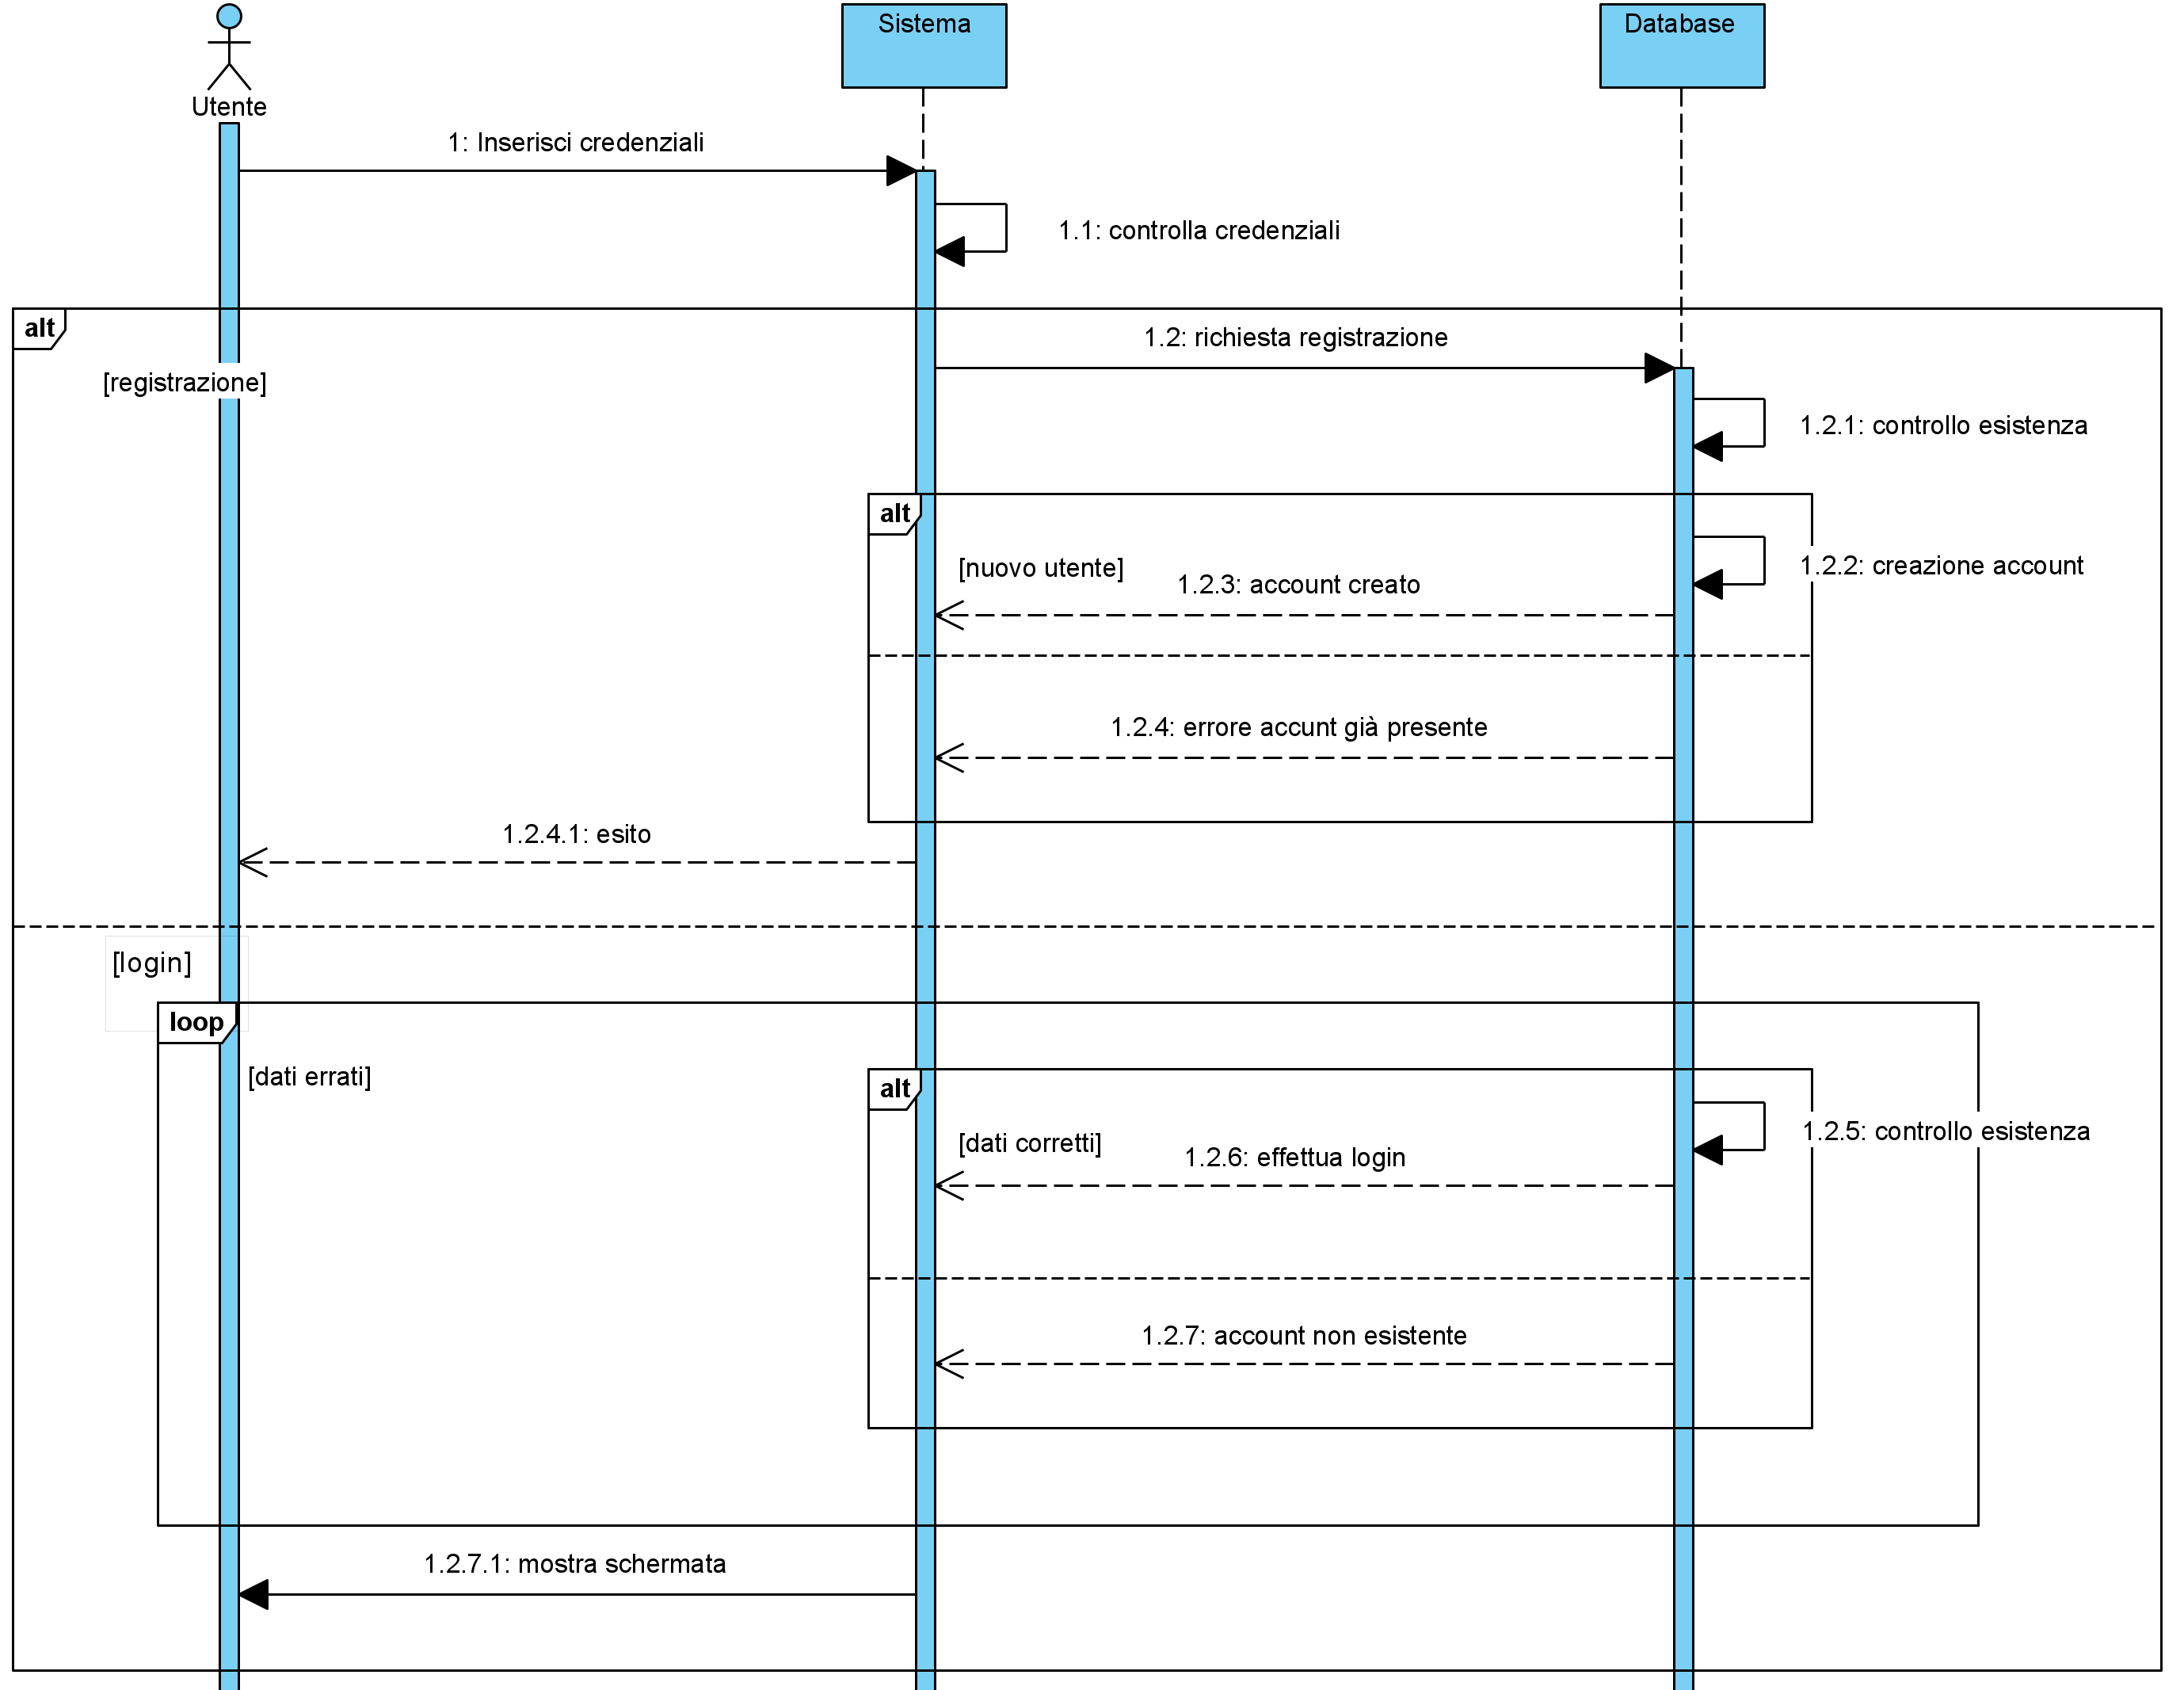
\includegraphics[scale=0.30]{Immagini/Sequence Diagram_Brew Day!_1.png}
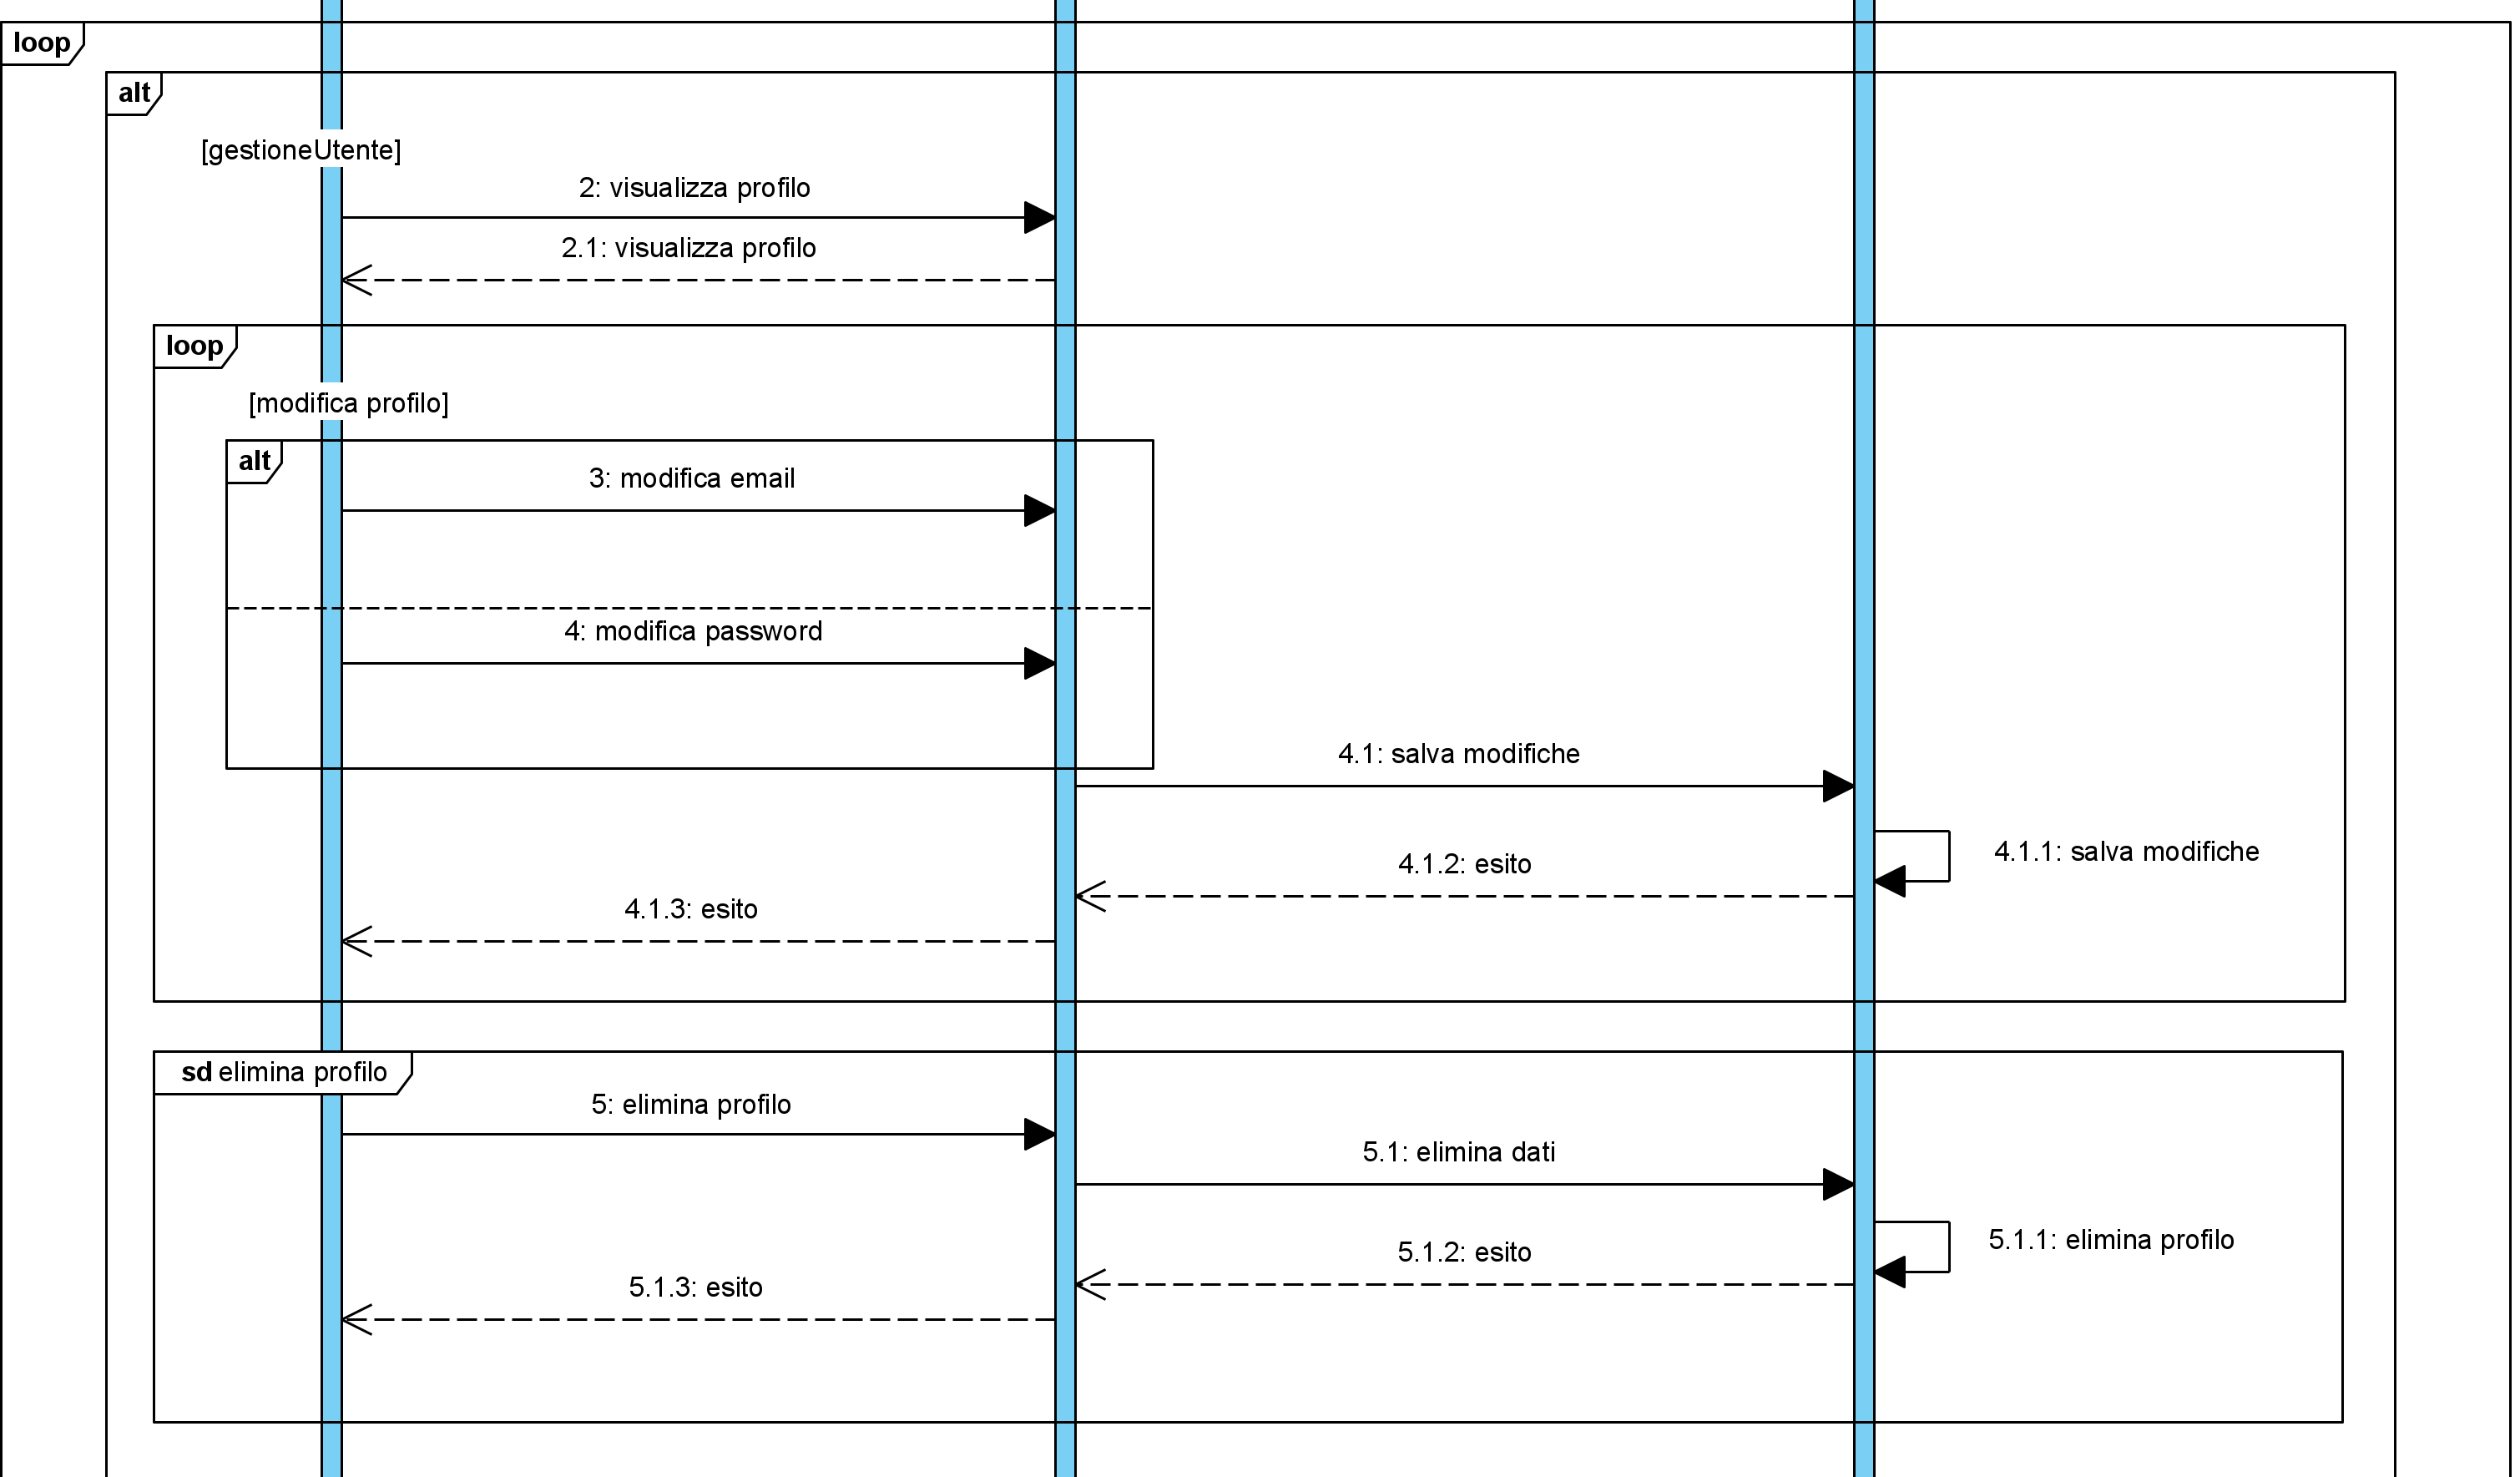
\includegraphics[scale=0.30]{Immagini/Sequence Diagram_Brew Day!_2.png}
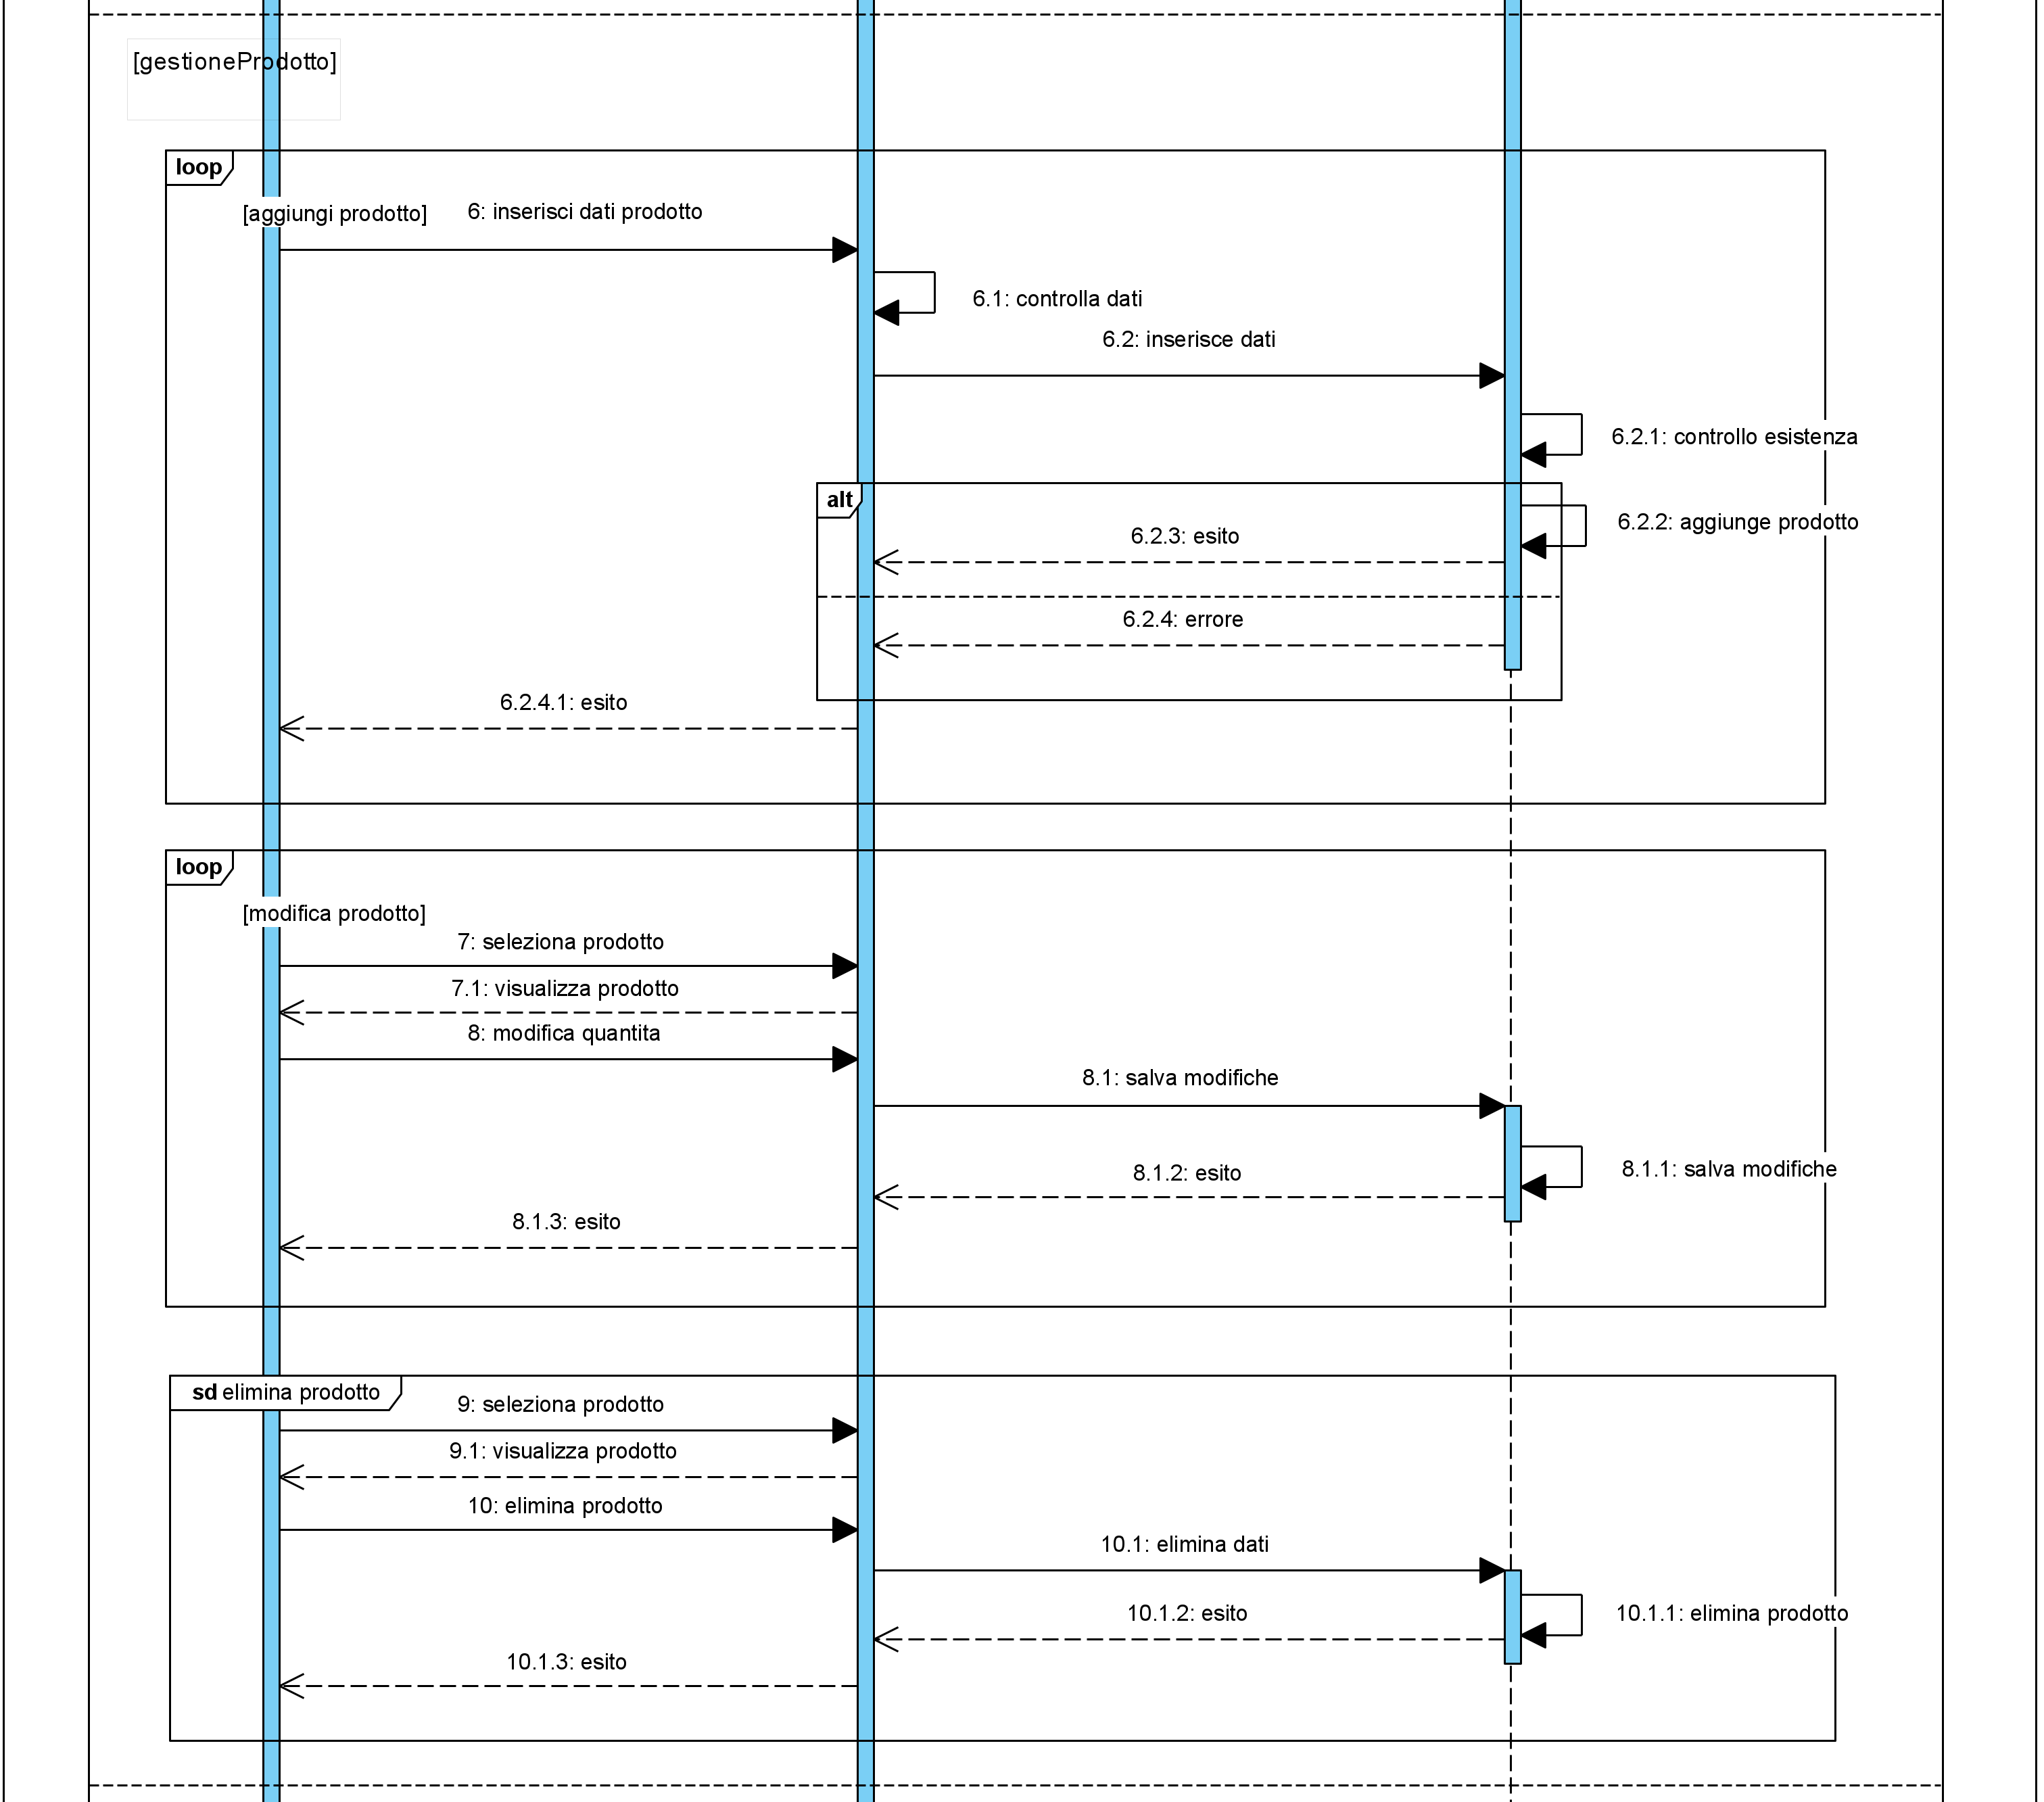
\includegraphics[scale=0.30]{Immagini/Sequence Diagram_Brew Day!_3.png}
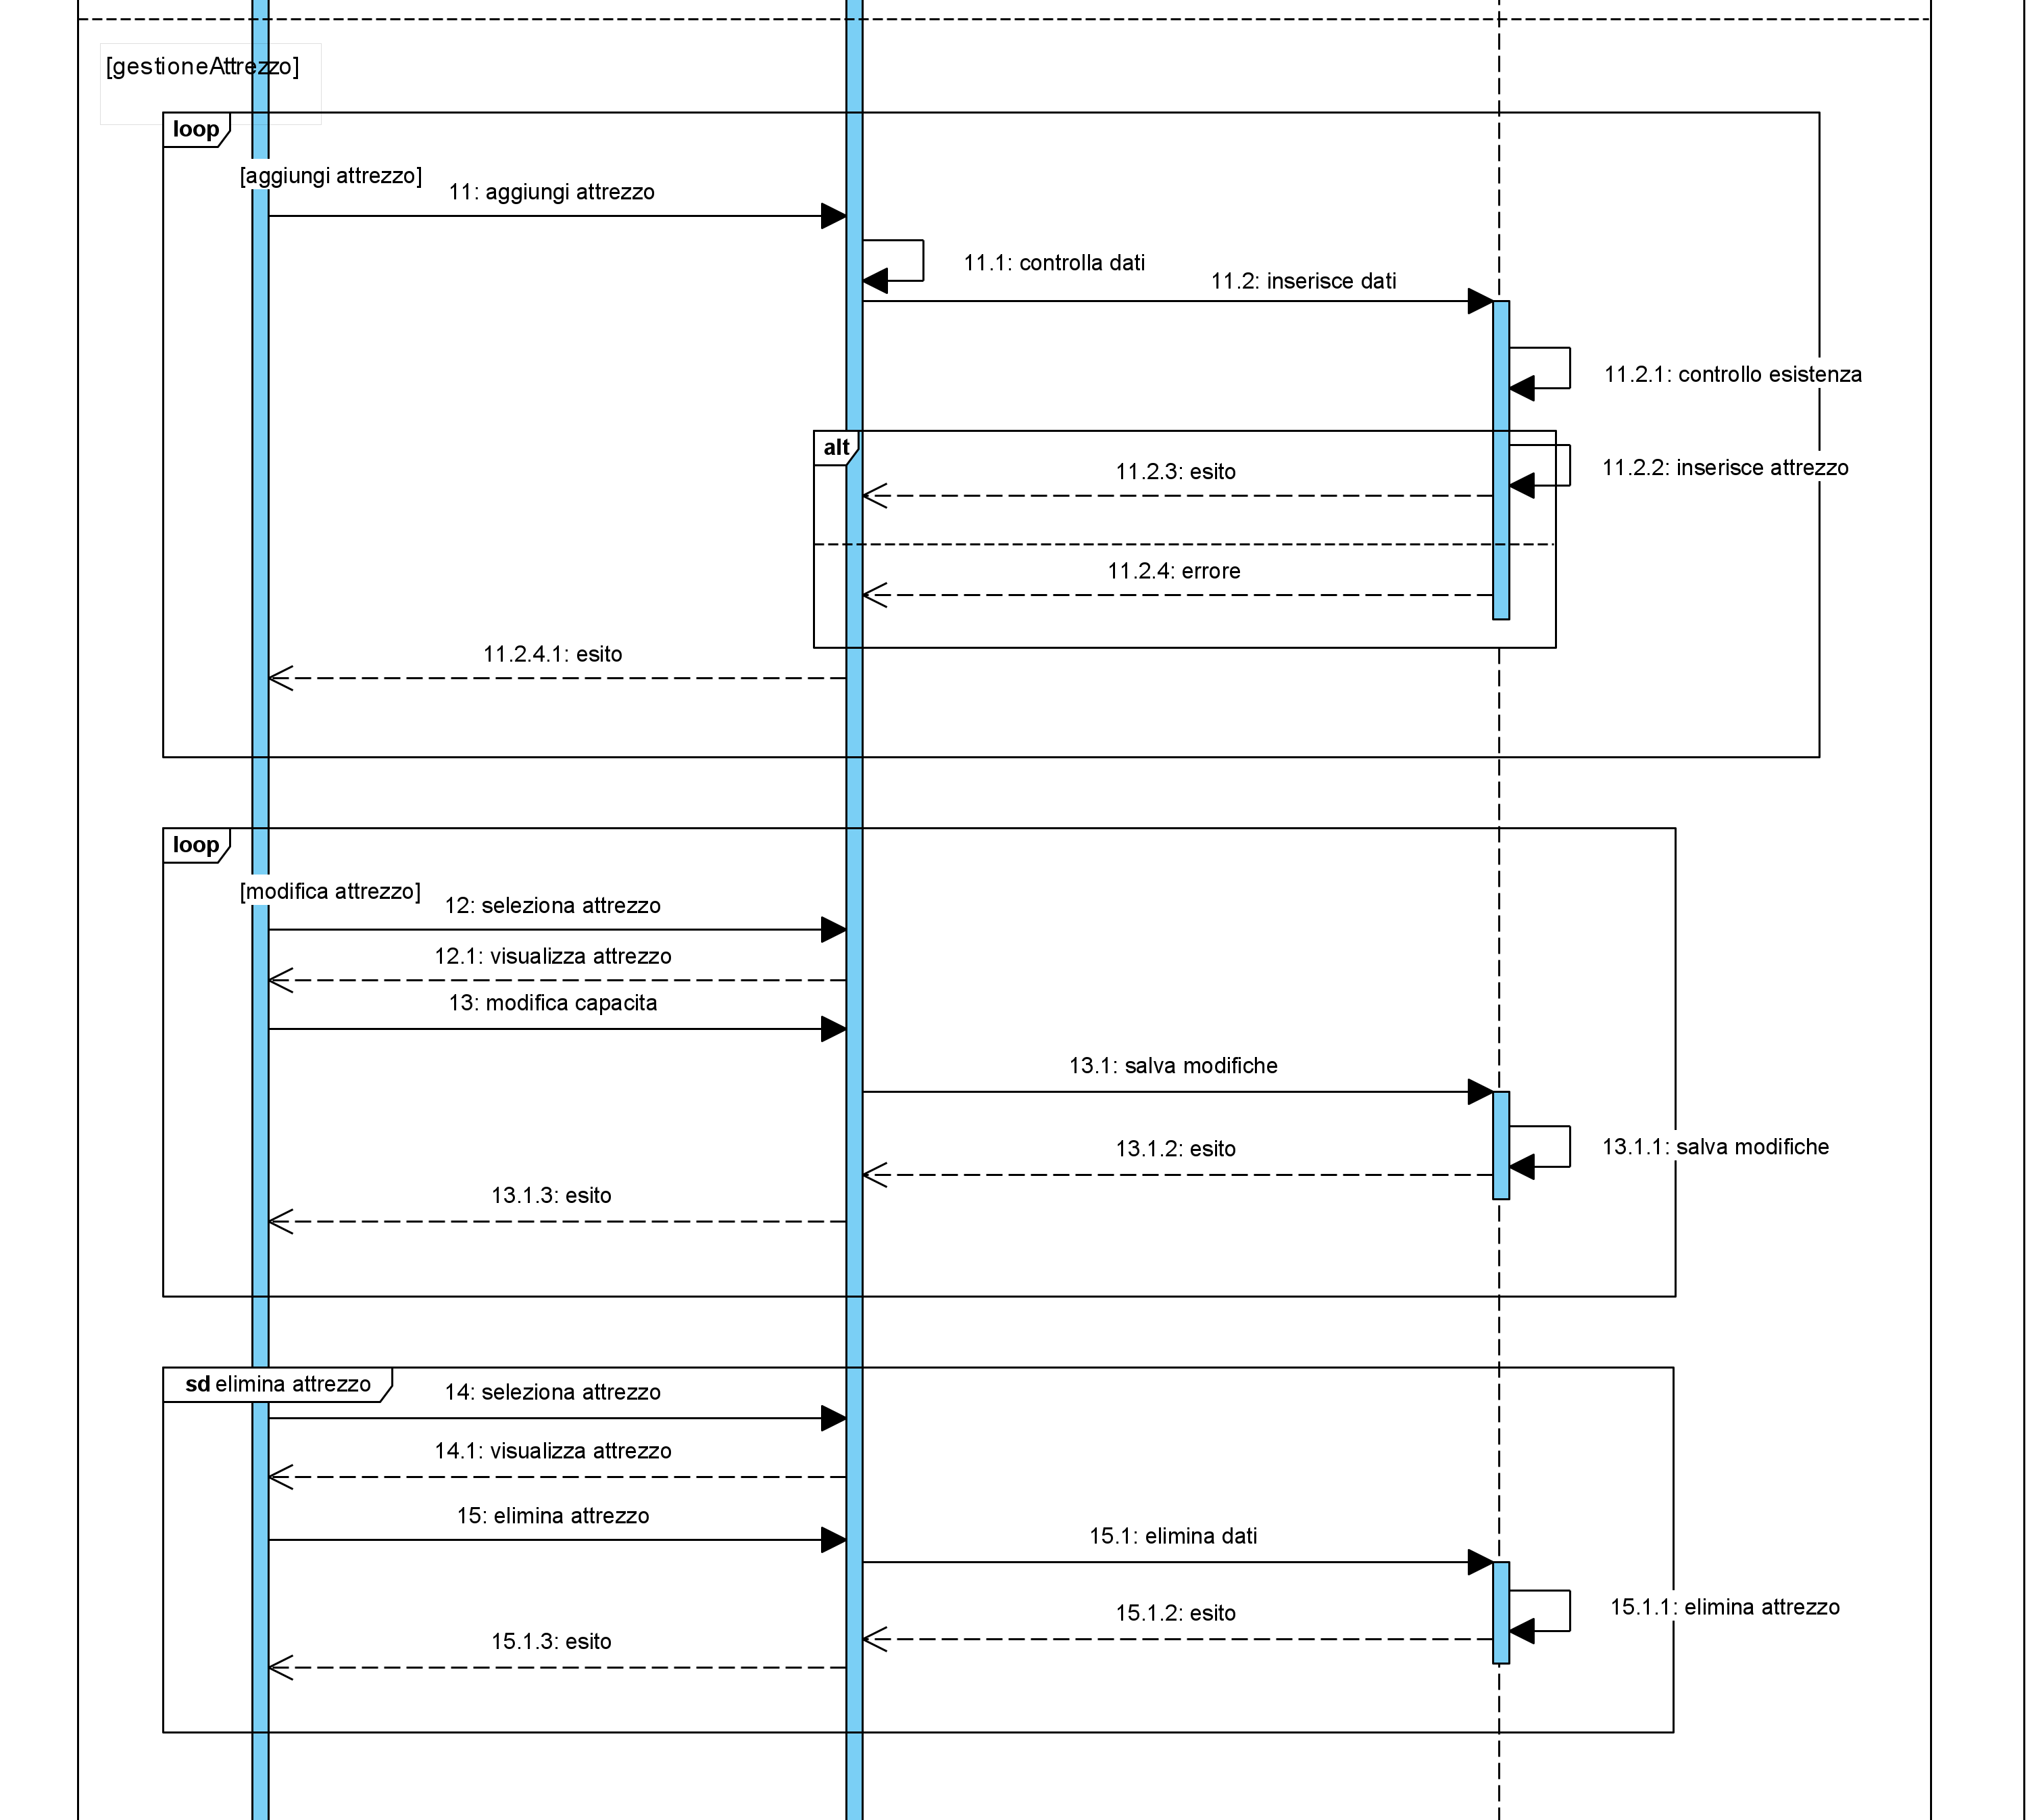
\includegraphics[scale=0.30]{Immagini/Sequence Diagram_Brew Day!_4.png}
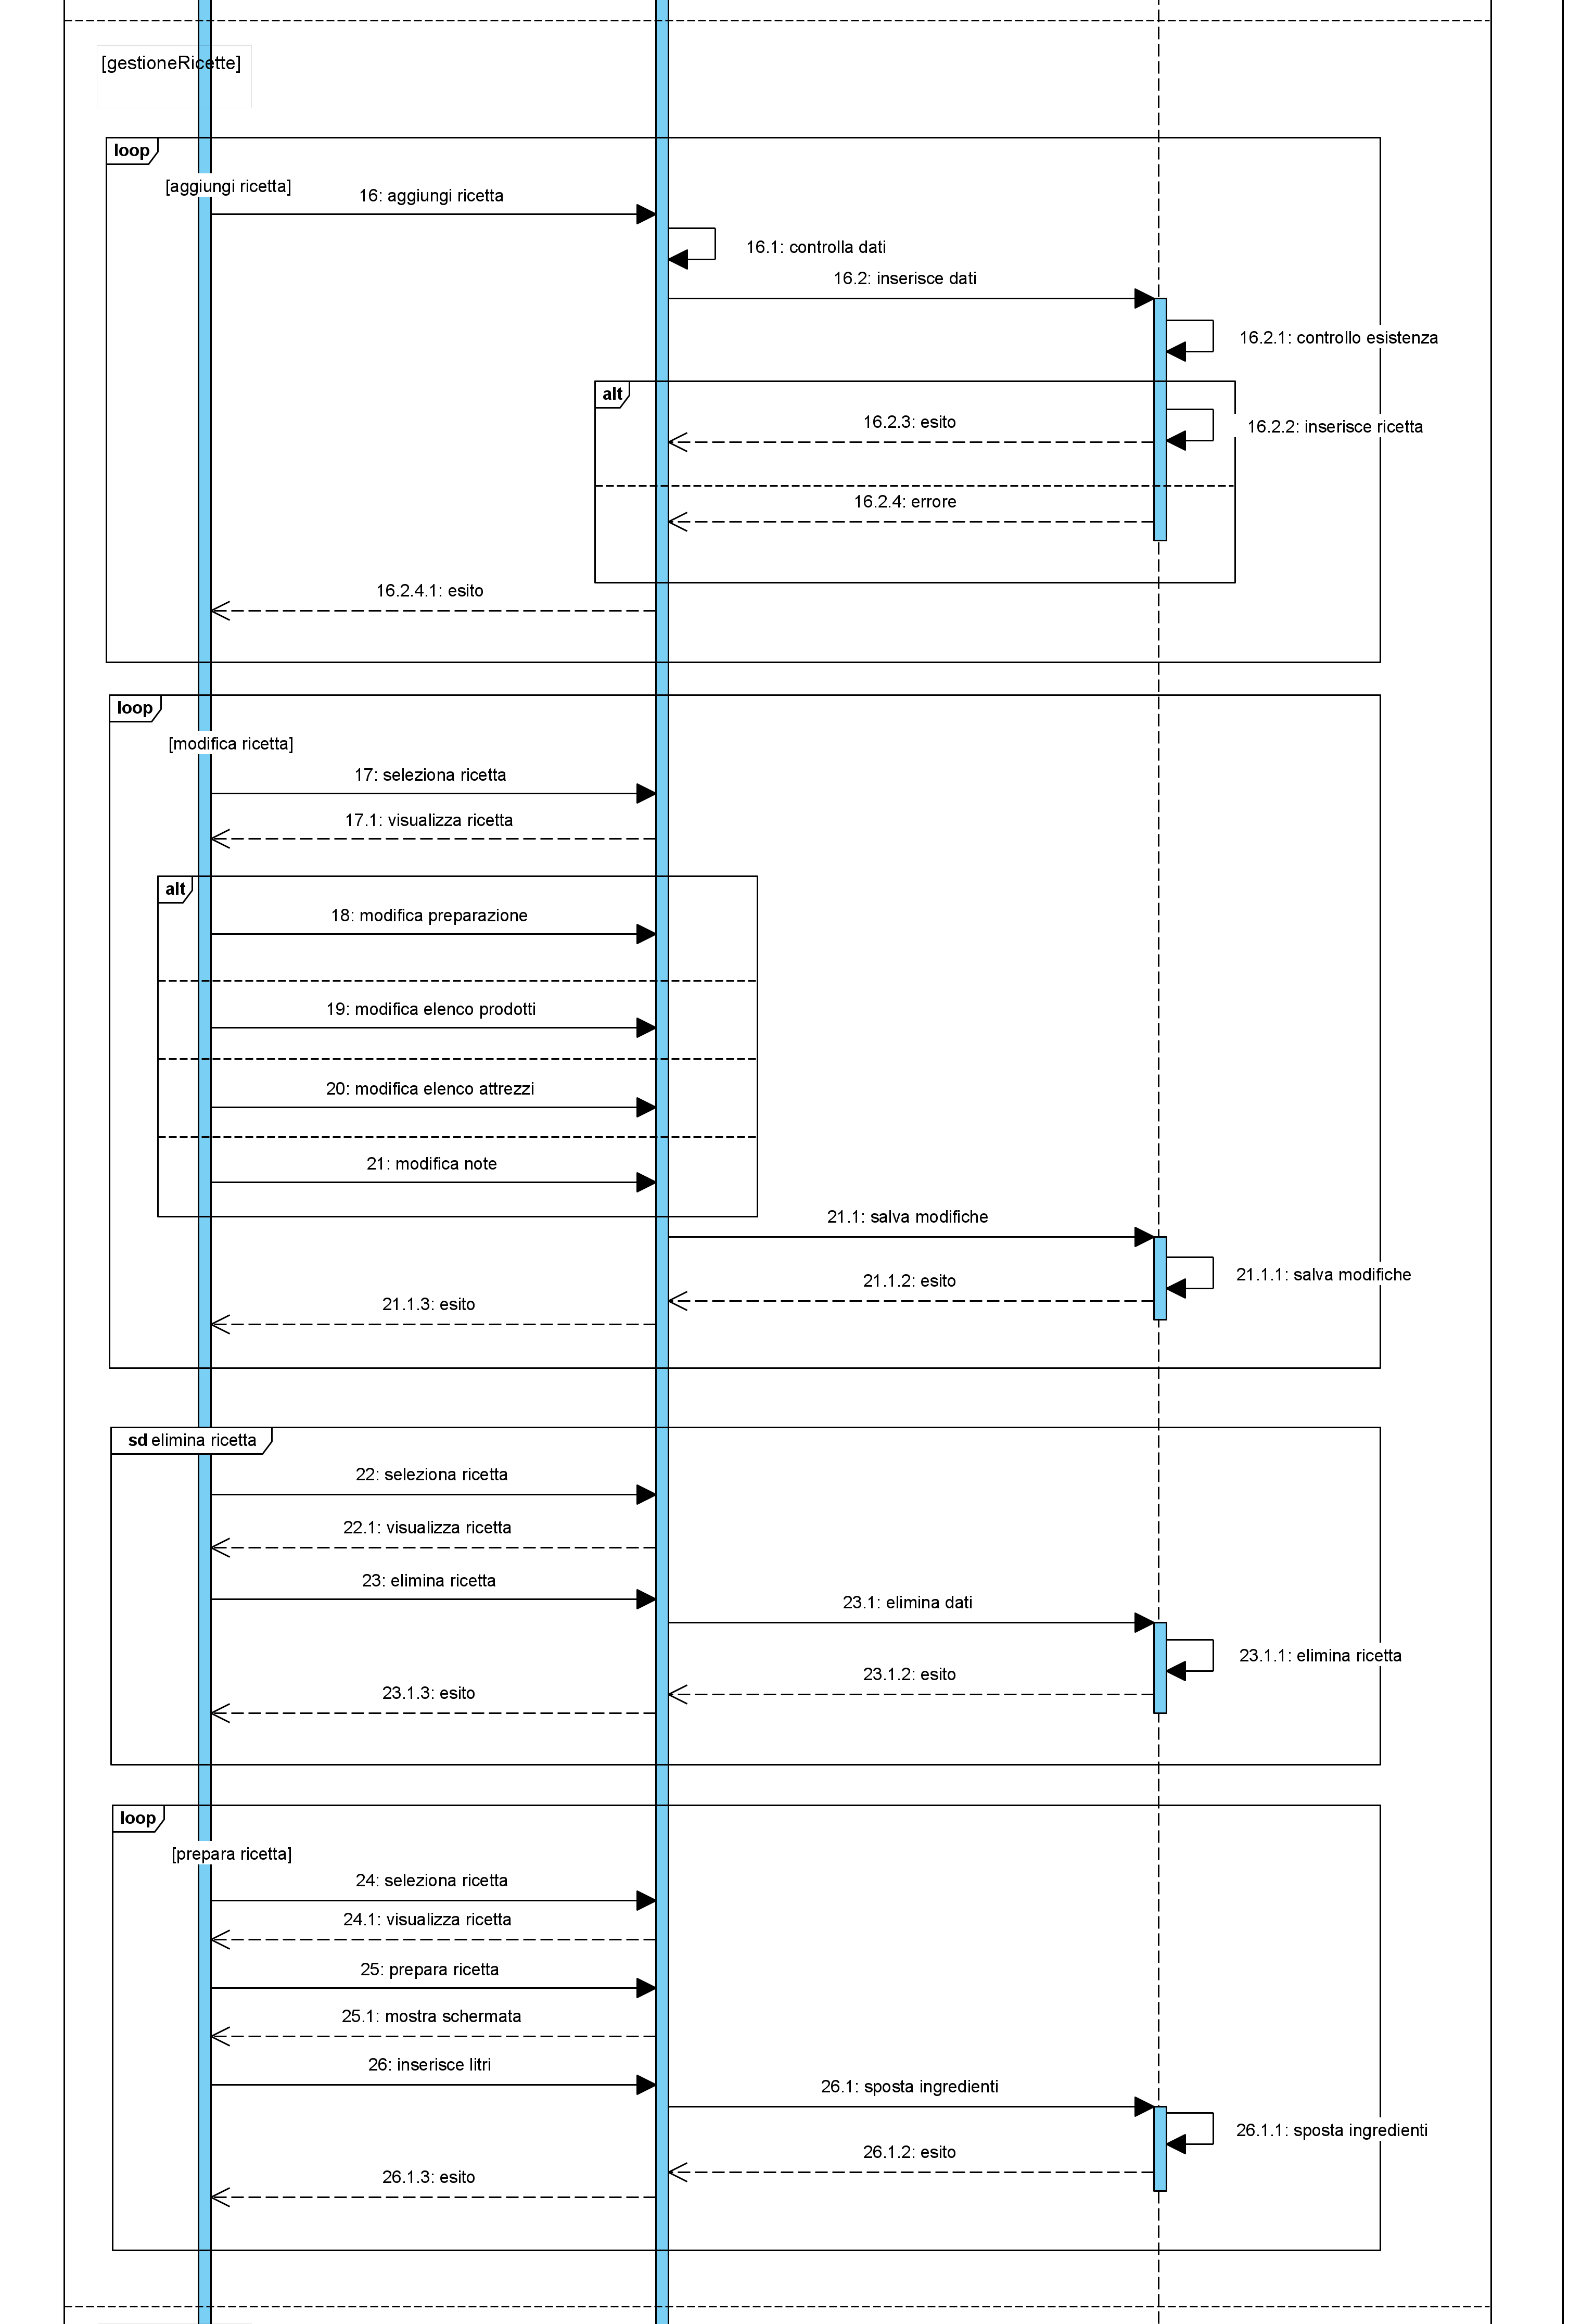
\includegraphics[scale=0.30]{Immagini/Sequence Diagram_Brew Day!_5.png}
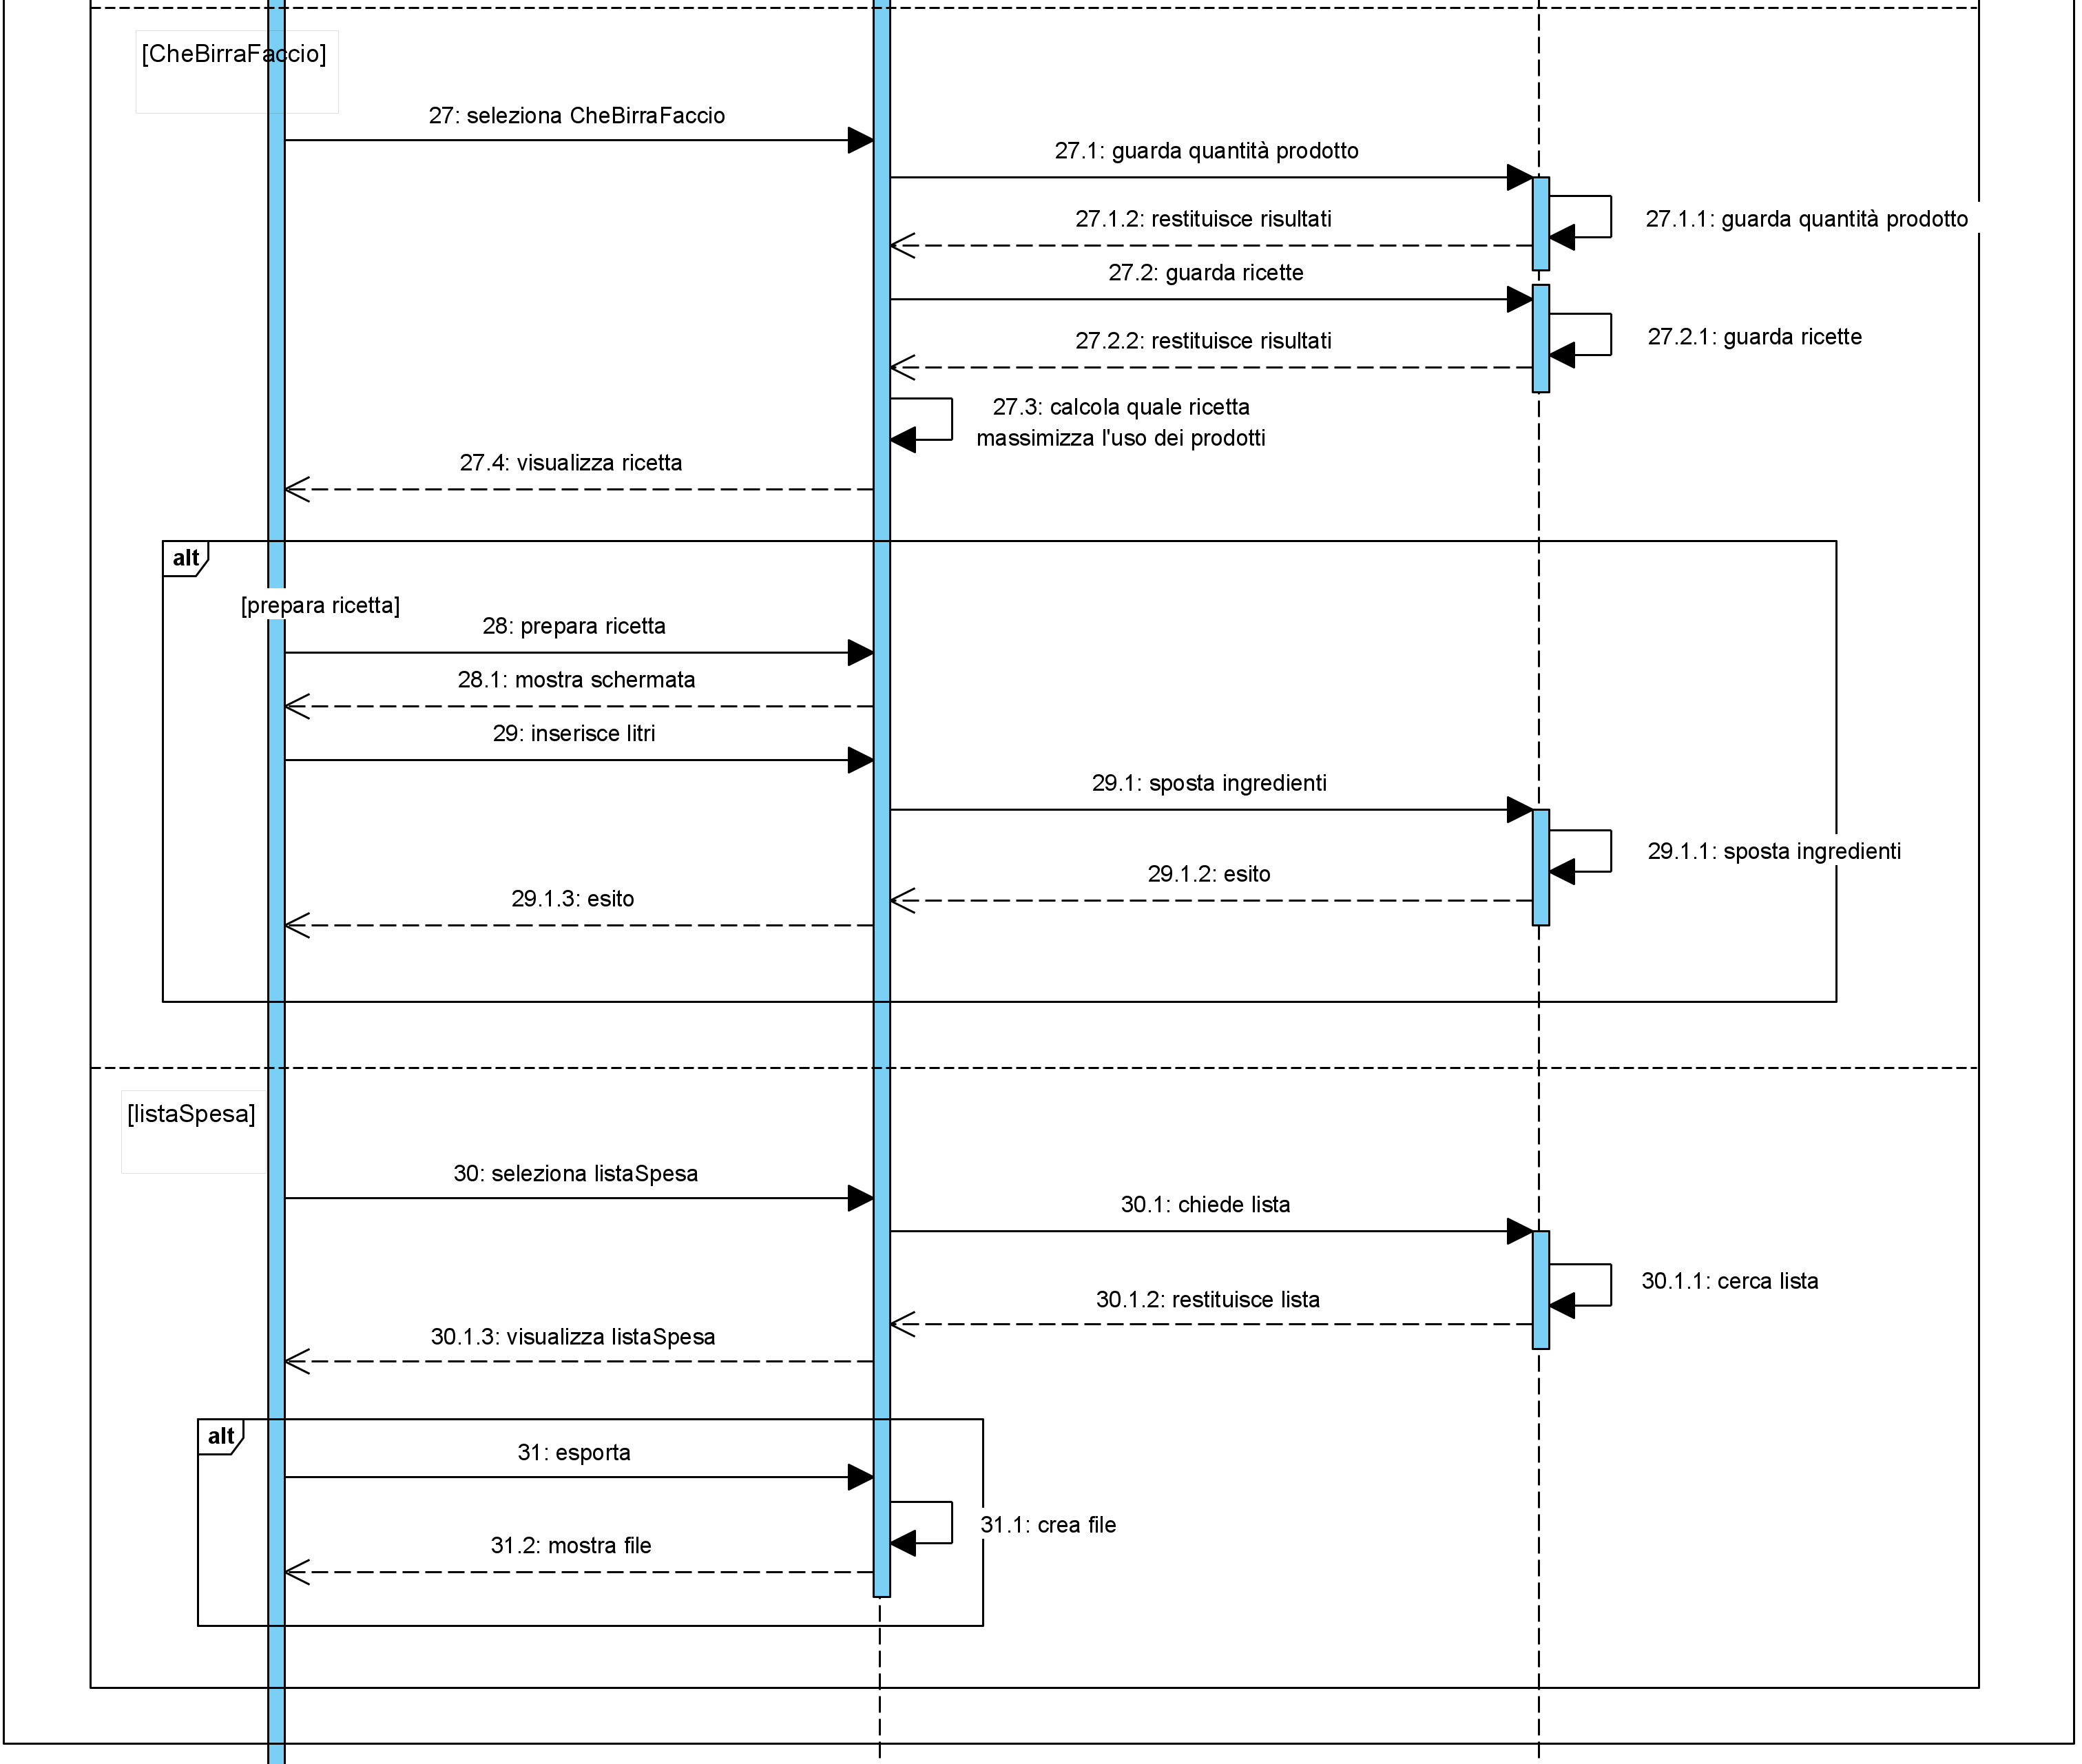
\includegraphics[scale=0.30]{Immagini/Sequence Diagram_Brew Day!_6.png}
\newpage
\section{Pattern}
\begin{comment}
\subsection{Pattern Grasp}
\subsubsection{Information Expert}
\subsubsection{Creator}
\subsubsection{Controller}
\subsubsection{Low Coupling}
\subsubsection{High Coesion}
\subsubsection{Protected Variations}
\end{comment}
\subsection{Singleton}
\subsection{Data Mapper}
\begin{comment}
\subsection{Identity Field}
\subsection{Association Table Mapping}
\end{comment}

\end{document}